% https://tex.stackexchange.com/questions/171982/how-to-make-table-floats-work-with-preview-standalone-environment/171983

\documentclass[%
    ,float=false % this is the new default and can be left away.
    ,preview=true
    ,class=scrartcl
%    ,fontsize=20pt
    ]{standalone}

\usepackage{amsmath}
\usepackage{tikz-dependency}
\DeclareMathOperator*{\argmax}{arg\,max}
\DeclareMathOperator*{\argmin}{arg\,min}
\DeclareMathOperator{\E}{\mathop{\mathbb{E}}}


\usepackage{helvet}
\renewcommand{\familydefault}{\sfdefault}

\usepackage{xcite}
\externalcitedocument{pnas-word-order-si}



\usepackage{footnote}
\makesavenoteenv{tabular}
\makesavenoteenv{table}

\usepackage{siunitx}

\usepackage{longtable}


\usepackage[numbers]{natbib}


\usepackage{amssymb}% http://ctan.org/pkg/amssymb
\usepackage{pifont}% http://ctan.org/pkg/pifont
\newcommand{\cmark}{\ding{51}}%
\newcommand{\xmark}{\ding{55}}%

\usepackage[english]{babel}
\usepackage[utf8]{inputenc}
\usepackage{bm}
\usepackage{graphicx}
\usepackage{tikz}
\usepackage{xcolor}
\usepackage{url}
\usepackage{rotating}
\usepackage{multirow}
\usepackage{natbib}
\usepackage{arydshln}

\newcommand{\key}[1]{\textbf{#1}}



\renewcommand{\thefigure}{S\arabic{figure}}
\renewcommand{\thetable}{S\arabic{table}}
\renewcommand{\thesection}{S\arabic{section}}



\usepackage{mathtools}
\DeclarePairedDelimiter{\ceiling}{\lceil}{\rceil}


\begin{document}
\begin{tabular}{|c|ll|c|cc|ccc}
	\hline
	%&
	&	\multicolumn{2}{c|}{Correlates with...}   &         \multirow{2}{*}{Real}   &  \multirow{2}{*}{Optimized} & \\ 
	&	verb & object     & & &   \\ 
	&	\emph{wrote} & \emph{letters} & & & \\ \hline \hline 
	\multirow{2}{*}{\raisebox{.5pt}{\textcircled{\raisebox{-.9pt} {1}}}}	&	adposition    &    noun phrase       
				&   \multirow{2}{*}{  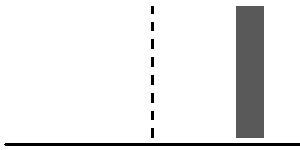
\includegraphics[width=0.12\textwidth]{figures/posterior_Real_lifted_case.pdf}     } 
		&   \multirow{2}{*}{  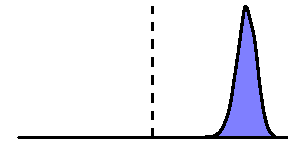
\includegraphics[width=0.12\textwidth]{figures/posterior_Efficiency_lifted_case.pdf}     } & \\
	&		\emph{to}            & \emph{a friend} &&&\\ \hline
	\multirow{2}{*}{\raisebox{.5pt}{\textcircled{\raisebox{-.9pt} {2}}}}	&copula    &    noun phrase         
		&   \multirow{2}{*}{  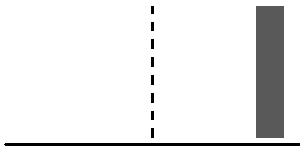
\includegraphics[width=0.12\textwidth]{figures/posterior_Real_lifted_cop.pdf}     } 
		&   \multirow{2}{*}{  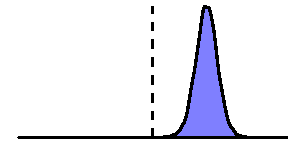
\includegraphics[width=0.12\textwidth]{figures/posterior_Efficiency_lifted_cop.pdf}     } & \\
	&	\emph{is}        & \emph{a friend}  &&&\\ \hline
	\multirow{2}{*}{\raisebox{.5pt}{\textcircled{\raisebox{-.9pt} {3}}}}	&auxiliary    &    verb phrase       
		&   \multirow{2}{*}{  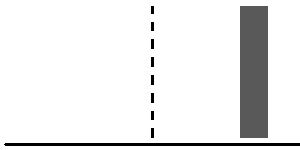
\includegraphics[width=0.12\textwidth]{figures/posterior_Real_aux.pdf}     } 
		&   \multirow{2}{*}{  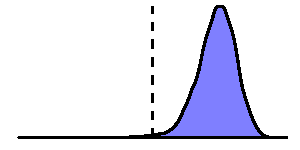
\includegraphics[width=0.12\textwidth]{figures/posterior_Efficiency_aux.pdf}     } & \\
	&	\emph{has}          & \emph{written}  &&&\\ \hline
	\multirow{2}{*}{\raisebox{.5pt}{\textcircled{\raisebox{-.9pt} {4}}}}	&noun    &    genitive      
		&   \multirow{2}{*}{  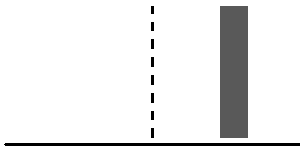
\includegraphics[width=0.12\textwidth]{figures/posterior_Real_nmod.pdf}     } 
		&   \multirow{2}{*}{  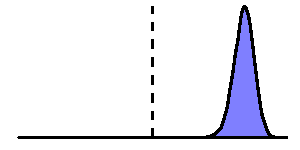
\includegraphics[width=0.12\textwidth]{figures/posterior_Efficiency_nmod.pdf}     } & \\
	&	\emph{friend} &  \emph{of John}  &&&\\ \hline
	\multirow{2}{*}{\raisebox{.5pt}{\textcircled{\raisebox{-.9pt} {5}}}}	&noun    &    relative clause      
		&   \multirow{2}{*}{  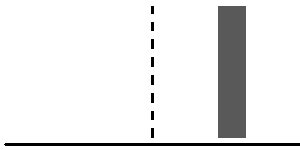
\includegraphics[width=0.12\textwidth]{figures/posterior_Real_acl.pdf}     } 
		&   \multirow{2}{*}{  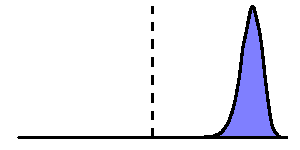
\includegraphics[width=0.12\textwidth]{figures/posterior_Efficiency_acl.pdf}     } & \\
	&	\emph{books} & \emph{that you read}  &&&\\ \hline
	\multirow{2}{*}{\raisebox{.5pt}{\textcircled{\raisebox{-.9pt} {6}}}}	&complementizer    &    sentence        
		&   \multirow{2}{*}{  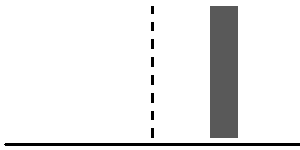
\includegraphics[width=0.12\textwidth]{figures/posterior_Real_lifted_mark.pdf}     } 
		&   \multirow{2}{*}{  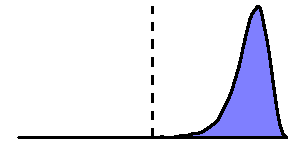
\includegraphics[width=0.12\textwidth]{figures/posterior_Efficiency_lifted_mark.pdf}     } & \\
	&	\emph{that} & \emph{she has arrived}  &&&\\ \hline
	\multirow{2}{*}{	\raisebox{.5pt}{\textcircled{\raisebox{-.9pt} {7}}}}	&verb    &    adp. phrase         
		&   \multirow{2}{*}{  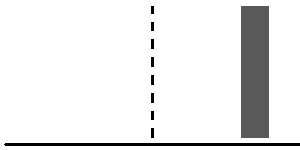
\includegraphics[width=0.12\textwidth]{figures/posterior_Real_obl.pdf}     } 
		&   \multirow{2}{*}{  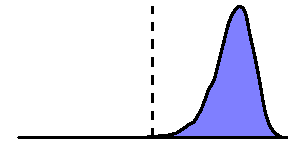
\includegraphics[width=0.12\textwidth]{figures/posterior_Efficiency_obl.pdf}     } & \\
	&	\emph{went} & \emph{to school}  &&&\\ \hline
	\multirow{2}{*}{\raisebox{.5pt}{\textcircled{\raisebox{-.9pt} {8}}}}	&want    &    verb phrase        
		&   \multirow{2}{*}{  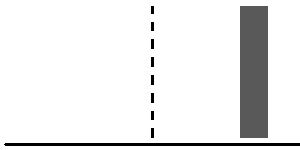
\includegraphics[width=0.12\textwidth]{figures/posterior_Real_xcomp.pdf}     } 
		&   \multirow{2}{*}{  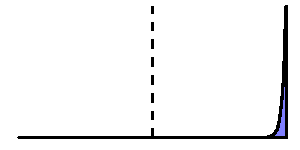
\includegraphics[width=0.12\textwidth]{figures/posterior_Efficiency_xcomp.pdf}     } & \\
	& \emph{wants}   &  \emph{to leave}  &&&\\ \hline
\end{tabular}
\end{document}

